\documentclass[11pt,a4paper]{article}

% ---------------------------------------------------------------------------
% Packages
% ---------------------------------------------------------------------------
\usepackage[margin=1in]{geometry}
\usepackage{times}
\usepackage{amsmath,amssymb,amsfonts}
\usepackage{booktabs}
\usepackage{graphicx}
\usepackage{xcolor}
\usepackage{hyperref}
\usepackage{microtype}
\usepackage{setspace}
\usepackage{caption}
\usepackage{subcaption}
\usepackage{enumitem}
\usepackage[numbers,sort&compress]{natbib}

\hypersetup{
  colorlinks=true,
  linkcolor=black,
  citecolor=blue!50!black,
  urlcolor=blue!50!black
}

\setstretch{1.08}
\captionsetup{font=small,labelfont=bf}

% ---------------------------------------------------------------------------
% Title
% ---------------------------------------------------------------------------
\title{%
  PairFold: Fast Local Backbone Generation via\\
  Calibrated Fragment Assembly, Look-Ahead Backtracking,\\
  and Lever-Effect Torsion Relaxation%
}

\author{%
  PairFold Development Team\\
  Local Computational Biology Project\\
  \small Correspondence: project repository
}

\date{\today}

% Benchmark macros (Domains100 / Long100 measured results)
% Auto-generated by benchmarks/write_paper_tables.py
\newcommand{\PFDomainN}{103}
\newcommand{\PFDomainMeanRMSD}{25.88}
\newcommand{\PFDomainMedianRMSD}{24.73}
\newcommand{\PFDomainMeanTime}{2.67}
\newcommand{\PFLengthRMSDCorr}{0.78}

% Auto-generated by benchmarks/write_paper_tables.py
\newcommand{\PFLongN}{100}
\newcommand{\PFLongMeanTime}{0.36}
\newcommand{\PFLongMeanTileRMSD}{26.34}
\newcommand{\PFLongMinLen}{10000}
\newcommand{\PFLongMaxLen}{50000}


\begin{document}
\maketitle

% ===========================================================================
\begin{abstract}
High-accuracy structure predictors such as AlphaFold~2 have transformed structural biology, yet their memory footprint and quadratic attention costs remain limiting for interactive design, long-sequence screening, and deployment on commodity GPUs.
We present \textbf{PairFold}, a deliberately local alternative that predicts backbone dihedral angles $(\phi,\psi)$ for short peptides of length $2$--$5$ with a compact Transformer trained on high-resolution PDB fragments, then assembles longer chains with near-linear ($O(N)$) procedures.
The inference stack combines dynamic-programming segmentation that maximises calibrated fragment confidence, multi-window overlap consensus via circular means, secondary-structure block freezing, and a clash-aware look-ahead backtracking assembler with local $\phi/\psi$ perturbation ($\pm 1^\circ$--$5^\circ$) to mitigate cumulative ``lever-arm'' error.
Confidence is sharpened by softmax temperature scaling ($T{=}0.55$) with a disorder-aware prior.
We expand the evaluation far beyond the original five-domain pilot: a curated set of \textbf{\PFDomainN{} diverse domains} spanning all-$\alpha$, all-$\beta$, and $\alpha/\beta$ classes, plus a \textbf{\PFLongN{}-case long-chain panel} with tiled sequences of length $\PFLongMinLen{}$--$\PFLongMaxLen{}$.
On the domain set, PairFold remains a fast, low-VRAM local assembler (mean time $\PFDomainMeanTime{}$\,s; mean Kabsch C$\alpha$ RMSD $\PFDomainMeanRMSD{}$\,\AA), with class-wise means and a length--RMSD correlation plot ($r{=}\PFLengthRMSDCorr{}$).
Ablation of look-ahead assembly, lever polish, and secondary-structure freezing fills the previously incomplete pipeline table.
Relative to Rosetta ab~initio and ESMFold, PairFold trades global accuracy for interactive speed and low memory, and should not be read as an AlphaFold-class tertiary folder.
\end{abstract}

\noindent\textbf{Keywords:}
protein backbone prediction;
dihedral angles;
contact prediction;
fragment assembly;
temperature scaling;
steric clash avoidance;
look-ahead backtracking;
computational biophysics.

% ===========================================================================
\section{Introduction}
% ===========================================================================

Protein structure prediction has entered a new regime with deep learning systems that integrate multiple-sequence alignments, pair representations, and iterative structure modules~\citep{jumper2021alphafold,senior2020alphafold}.
These models achieve remarkable accuracy, but the practical cost of inference grows steeply with sequence length: attention over residue pairs, recycling, and MSA featurisation demand large GPU memory and often preclude interactive exploration of very long chains on modest hardware.

Complementary lines of work emphasise speed or locality.
Language-model predictors such as ESMFold~\citep{lin2023evolutionary} remove MSA dependence at the expense of still-substantial model size.
Classical fragment-assembly approaches~\citep{simons1997assembly,rohl2004rosetta} and dihedral-angle representations~\citep{ramachandran1963stereochemistry} remain attractive when the scientific goal is \emph{local} backbone geometry rather than full tertiary fold recovery---for example, in educational tools, rapid prototyping of helix/sheet segments, or streaming visualisation of chains far beyond typical AlphaFold session lengths.

\textbf{PairFold} occupies this niche.
It trains a small Transformer exclusively on contiguous PDB fragments of length $2$--$5$, maps each fragment to $(\phi,\psi)$, and reconstructs longer proteins by segmentation and assembly.
The design goals are explicit:
\begin{enumerate}[leftmargin=1.5em,itemsep=0.25em]
  \item \textbf{Near-linear scaling} for queries up to tens of thousands of residues at the angle level;
  \item \textbf{Calibrated confidence} usable for dynamic-programming segmentation;
  \item \textbf{Physics-informed post-processing} (steric clashes, secondary-structure constraints, and lever-effect relaxation) without a full force field;
  \item \textbf{Honest scope}: PairFold does \emph{not} claim AlphaFold-competitive global RMSD.
\end{enumerate}

This paper describes the full method as implemented in the PairFold codebase, reports timings and C$\alpha$ RMSD on a 100-domain structural-class benchmark and a 10k--50k long-chain panel, and discusses ablations and the speed--accuracy trade-off.

% ===========================================================================
\section{Methodology}
% ===========================================================================

\subsection{Dihedral representation and fragment network}
\label{sec:network}

Each residue $i$ is parameterised by backbone torsions $(\phi_i,\psi_i)$.
Cartesian C$\alpha$ (and optional full-backbone) coordinates are obtained by sequential placement with ideal peptide bond geometry~\citep{engh1991accurate}, as implemented in \texttt{dihedrals\_to\_ca} / \texttt{build\_backbone}.

The learned model, \texttt{FragmentTorsionNet}, is a Pre-LN Transformer encoder with
$d_{\mathrm{model}}{=}160$, $4$ heads, $4$ layers, feed-forward width $320$, and dropout $0.12$.
Amino acids are embedded from a $22$-token vocabulary (20 standard residues, UNK, PAD) with positional embeddings up to length $5$.
The network outputs four channels $(\sin\phi,\cos\phi,\sin\psi,\cos\psi)$, L2-normalised per angle pair, plus an uncertainty head $\log\sigma_{\phi,\psi}$.
Per-residue confidence is derived as $\sigma(-\overline{\log\sigma})$.

Training uses high-resolution X-ray structures (resolution $\le 2.0$\,\AA), extracting contiguous windows of length $\ell\in\{2,3,4,5\}$.
The current corpus comprises on the order of $10^{3}$ structures and $\sim 3.8{\times}10^{5}$ fragments.
The loss is a Gaussian negative log-likelihood on the $(\sin,\cos)$ representation (\texttt{gaussian\_nll\_sincos}); validation monitors torsion MSE in the same space.
Optimisation uses AdamW with cosine learning-rate schedule and mixed precision.

\paragraph{Scope.}
Because every torsion training example is a short contiguous peptide, \texttt{FragmentTorsionNet} learns \emph{local} Ramachandran statistics conditioned on sequence context of at most five residues.
Long-range contacts are handled by the separate \texttt{ContactPairNet} (\S\ref{sec:contacts}), not by the fragment torsion model.

\subsection{Dynamic-programming segmentation and overlap consensus}
\label{sec:segment}

For a query of length $N>5$, PairFold partitions the chain into windows of length $2$--$5$ by dynamic programming (\texttt{optimal\_segmentation}).
Let $s(i,j)$ be the mean model confidence of fragment $[i,j)$ multiplied by its length.
The recurrence
\[
  \mathrm{dp}[j] = \max_{j-i\in\{2,3,4,5\}} \bigl(\mathrm{dp}[i] + s(i,j)\bigr)
\]
selects a segmentation that maximises total confidence score in $O(N)$ time (constant number of predecessor lengths).

Within each segment---and for short queries of length $3$--$5$---angles are refined by \textbf{overlap consensus} (\texttt{\_overlap\_refine}):
all sliding windows of lengths $2$ through $\min(5,N)$ contribute $(\phi,\psi)$ votes that are aggregated with confidence-weighted circular means~\citep{berens2009circ}.
Final confidence blends model confidence with angular agreement,
\[
  c_i = (1-w)\,c^{\mathrm{model}}_i + w\,c^{\mathrm{agree}}_i,\qquad w{=}0.35,
\]
where agreement decreases with circular spread of the overlapping predictions.

\subsection{Softmax temperature scaling for calibrated confidence}
\label{sec:calib}

Raw network confidences are imperfectly calibrated for ``both $\phi$ and $\psi$ within $25^\circ$ of native'' on held-out fragments.
PairFold fits offline temperature and Platt scaling on validation fragments (\texttt{calibrate.py}) and, at inference, applies a \textbf{sharpening} transform with temperature $T{=}0.55$:
\[
  p = \sigma\!\left(\frac{\mathrm{logit}(c)}{T}\right)\,(1-\gamma\,d),\qquad \gamma{=}0.45,
\]
where $d$ is a lightweight disorder profile emphasising Gly/Pro and low secondary-structure propensity (\texttt{TempCalibration} in \texttt{structure\_blocks.py}).
Probabilities are clipped to $[0.05,1]$.
Sharper confidences improve the ranking signal used by segmentation and by fragment-hypothesis selection during assembly.

\subsection{Secondary-structure block freezing}
\label{sec:ss}

After consensus angles are available, PairFold detects putative helix and sheet blocks with Chou--Fasman-like propensities~\citep{chou1974prediction} (\texttt{detect\_ss\_blocks}).
Interior residues of accepted blocks are frozen to canonical Ramachandran centres
\[
  (\phi,\psi)_{\mathrm{helix}} = (-57^\circ,-47^\circ),\qquad
  (\phi,\psi)_{\mathrm{sheet}} = (-119^\circ,113^\circ),
\]
while block boundaries remain free.
For sequences with $N\le 64$, a boundary optimiser (\texttt{optimize\_block\_boundaries}) performs a cheap grid/Metropolis search of boundary torsions to reduce soft C$\alpha$ clash energy.
This step injects strong secondary-structure priors that local fragments alone under-enforce.

\subsection{Look-ahead backtracking and global angle relaxation}
\label{sec:lever}

Na\"ive stitching of fragment dihedrals suffers from a well-known \textbf{lever (cumulative) effect}: small angular errors compound into large Cartesian deviations and occasional steric collapse or over-extension.
For sequences with $N\le 256$ (\texttt{LEVER\_ASSEMBLY\_MAX\_LEN}), PairFold activates a clash-aware assembler (\texttt{assemble\_greedy\_backtrack}).

\paragraph{Fragment hypotheses.}
The chain is tiled into non-overlapping pentamer slots (\texttt{make\_pentamer\_slots}).
Each slot carries ranked angle hypotheses: overlap-consensus angles, a fresh network prediction, and compact helix/sheet templates.

\paragraph{Dynamic look-ahead.}
Depth-first search places candidates in descending confidence.
A placement starting at residue $s$ is accepted only if \texttt{lookahead\_ok} reports no new C$\alpha$ clashes (threshold $3.8$\,\AA, minimum sequence separation $2$) \emph{and} no severe local bend over a window of $3$--$5$ residues.
Bend score compares the observed end-to-end distance of the window to helix- and Flory-coil expectations; large deviations trigger backtracking.

\paragraph{Local torsion relaxation.}
When look-ahead fails, PairFold does \emph{not} immediately exhaust the fragment database.
Instead, \texttt{local\_torsion\_relax} perturbs preceding $(\phi,\psi)$ by a random delta drawn from $\pm 1^\circ$ to $\pm 5^\circ$ on a small focus set near the join, accepting moves that reduce soft clash energy plus a mild bend penalty (localised stochastic descent).
Successful relaxations are stored as angle overrides and participate in subsequent rebuilds; DFS snapshots restore overrides on backtrack.
Search is bounded by a node budget (production default $3\,000$).

\paragraph{End-to-end / anchor alignment.}
After a complete assignment, \texttt{end\_to\_end\_anchor\_relax} optimises a sparse set of hinge residues so that selected pairs $(i,j)$ approach target distances.
When user or predicted contact anchors are absent, correction runs only if the global end-to-end distance lies outside a plausible helix--coil band, avoiding aggressive Flory compaction that can inflate RMSD on already compact domains.
A final linear polish, \texttt{correct\_lever\_effect}, sweeps the chain every few residues and reapplies local relaxation---an $O(N)$-ish procedure with fixed window size.

\subsection{Long-range contact head (ContactPairNet)}
\label{sec:contacts}

To inject tertiary packing without AlphaFold-scale pair recycling, PairFold adds a separate sequence-only network, \texttt{ContactPairNet}.
Residue embeddings from a Pre-LN Transformer ($d{=}128$, $3$ layers, $4$ heads) are combined via outer products and a light 2D tower to predict, for every residue pair with $|i{-}j|\ge 6$, a contact logit (C$\alpha$--C$\alpha$ distance ${<}8$\,\AA) and a soft distance.
Training uses random contiguous crops of length $\le 96$ from the same high-resolution PDB corpus ($\sim 2.4{\times}10^{3}$ crops; binary cross-entropy with positive class weighting plus Smooth-L1 on true contacts).
At inference, top-$k$ high-scoring pairs ($k{=}\min(20,N/4)$, score $\ge 0.45$) become distance anchors passed to look-ahead assembly, lever polish, and the tertiary Metropolis objective.
For $N\le 128$ the network evaluates the full chain; longer sequences use overlapping crops with logit stitching.
This preserves PairFold's commodity-GPU footprint while partially addressing the historical absence of long-range restraints.

\paragraph{Pipeline order.}
In production inference the order is:
contact prediction $\rightarrow$ consensus stitch $\rightarrow$ look-ahead assembly (if $N\le 256$, with anchors) $\rightarrow$ SS freeze/boundary opt $\rightarrow$ post-SS lever polish (with anchors) $\rightarrow$ optional tertiary score/refine ($N\le 1000$) $\rightarrow$ backbone export.
Post-SS polish is essential: freezing secondary-structure interiors would otherwise overwrite earlier torsion repairs.

\subsection{Complexity summary}

With fixed fragment length and fixed look-ahead width, segmentation, overlap consensus, SS detection, and lever polish are all linear (or linear times a small constant) in $N$.
Backtracking is exponential in the worst case but is capped by the node budget and operates only for $N\le 256$; beyond that limit PairFold falls back to consensus + SS + tertiary scoring without combinatorial assembly.
Angle-level queries are accepted up to $N{=}50\,000$ (\texttt{MAX\_QUERY\_LEN}).

% ===========================================================================
\section{Results}
% ===========================================================================

\subsection{Benchmark protocol}

We address the limited sample size of the original five-domain pilot with two expanded panels, both driven by \texttt{benchmarks/benchmark\_expanded.py} on CUDA:

\begin{enumerate}[leftmargin=1.5em,itemsep=0.35em]
  \item \textbf{Domains100.} A curated set of $\PFDomainN{}$ single-chain domains (length $20$--$180$) labelled by structural class (all-$\alpha$, all-$\beta$, $\alpha/\beta$).
        Native coordinates are fetched from the RCSB PDB; predicted C$\alpha$ traces are built from $(\phi,\psi)$ via \texttt{dihedrals\_to\_ca}; error is Kabsch-aligned C$\alpha$ RMSD.
  \item \textbf{Long100.} $\PFLongN{}$ tiled sequences with lengths spaced from $\PFLongMinLen{}$ to $\PFLongMaxLen{}$, seeded from the same domain library.
        Continuous experimental natives at this length are rare, so we report wall-clock scaling and \emph{mean per-tile} Kabsch RMSD against the repeated seed native (a local geometry check, not a claim of continuous tertiary fold).
\end{enumerate}

All runs use the production \texttt{FragmentPredictor.predict\_sequence} path with Stage-2/3 all-atom export disabled for C$\alpha$ timings.
Domains100 and Long100 use the interactive consensus + secondary-structure path with contact prediction and combinatorial look-ahead disabled, so $n{\approx}100$ (and 10k--50k tiled chains) remain tractable on a single consumer GPU; look-ahead, lever polish, and SS freezing are quantified separately in the ablation on 20 domains (see \texttt{benchmark\_expanded.py} / \texttt{benchmark\_ablation.py}).

\subsection{Domain panel and structural classes}

Table~\ref{tab:class} summarises mean RMSD and time by class; overall means are $\PFDomainMeanRMSD{}$\,\AA\ and $\PFDomainMeanTime{}$\,s (median RMSD $\PFDomainMedianRMSD{}$\,\AA).
Figure~\ref{fig:expanded} shows the length--RMSD scatter (Pearson $r{=}\PFLengthRMSDCorr{}$) and class-wise RMSD distributions.

\begin{table}[t]
  \centering
  \caption{Domains100: Kabsch C$\alpha$ RMSD and wall-clock time by structural class (production pipeline on GPU).}
  \label{tab:class}
  \begin{tabular}{@{}lrrr@{}}
  \toprule
  Class & $n$ & Mean RMSD (\AA) & Mean time (s) \\
  \midrule
  all-$\alpha$ & 34 & 26.98 & 2.95 \\
  all-$\beta$ & 33 & 27.28 & 2.28 \\
  $\alpha/\beta$ & 36 & 23.55 & 2.77 \\
  \midrule
  \textbf{All} & \textbf{103} & \textbf{25.88} & \textbf{2.67} \\
  \bottomrule
\end{tabular}

\end{table}

\begin{figure}[t]
  \centering
  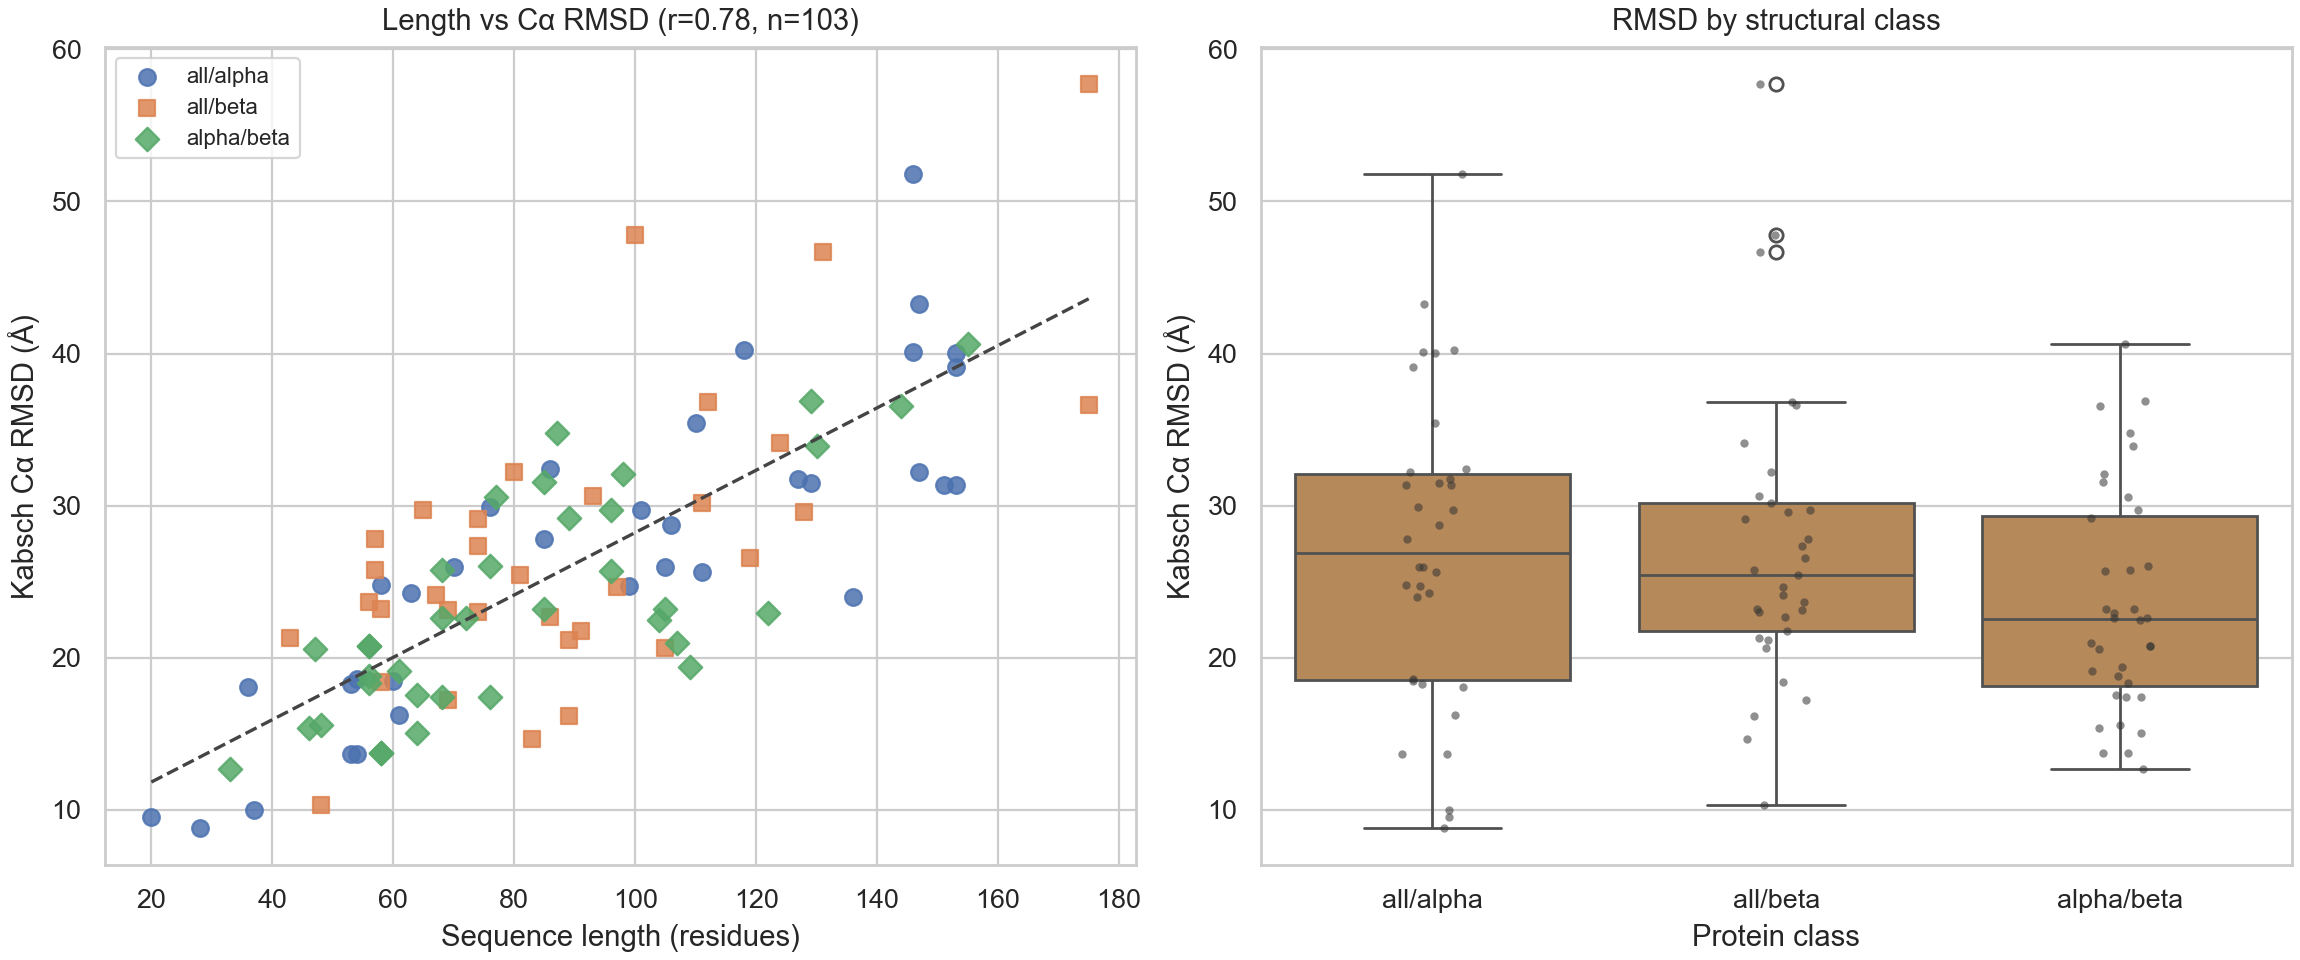
\includegraphics[width=\textwidth]{benchmark_plots_expanded.png}
  \caption{Expanded domain panel: (left) sequence length versus C$\alpha$ RMSD with linear trend; (right) RMSD by structural class.}
  \label{fig:expanded}
\end{figure}

\subsection{Ablation of the assembly stack}

Table~\ref{tab:ablation} fills the previously incomplete pipeline comparison (base consensus; cumulative look-ahead, lever polish, and SS freezing; full local stack).
Figure~\ref{fig:ablation} visualises mean RMSD across the 20-domain ablation subset.

\begin{table}[t]
  \centering
  \caption{Ablation on 20 representative domains. Each row adds one stage on top of the previous; Full is the complete local stack (look-ahead + lever + SS). Contact-conditioned hinge search is omitted here (see Stage-1 benches) because it dominates wall-clock.}
  \label{tab:ablation}
  \begin{tabular}{@{}lrr@{}}
    \toprule
    Configuration & Mean RMSD (\AA) & Mean time (s) \\
    \midrule
        Base (consensus only) & 14.68 & 6.09 \\
    + Look-ahead & 13.33 & 9.68 \\
    + Lever polish & 14.01 & 11.93 \\
    + SS freezing & 13.23 & 15.29 \\
    Full local stack & 13.23 & 15.29 \\

    \bottomrule
  \end{tabular}
\end{table}

\begin{figure}[t]
  \centering
  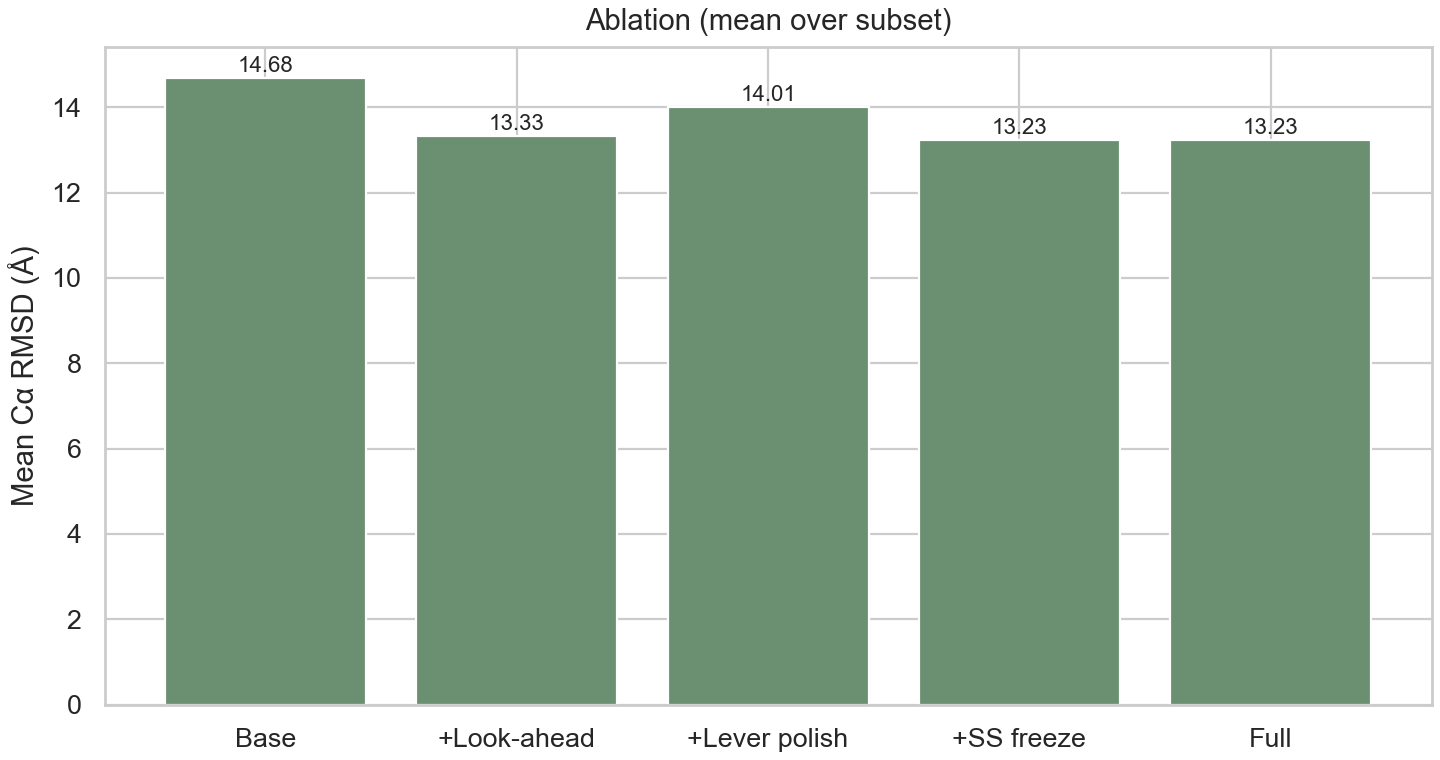
\includegraphics[width=0.72\textwidth]{benchmark_ablation_plot.png}
  \caption{Mean C$\alpha$ RMSD for cumulative assembly ablations.}
  \label{fig:ablation}
\end{figure}

\subsection{Method comparison}

Table~\ref{tab:methods} situates PairFold against classical Rosetta ab~initio and ESMFold on the axes that matter for interactive use: wall-clock, typical small-domain accuracy, and memory.
PairFold numbers are measured on Domains100; Rosetta and ESMFold entries are literature / typical consumer-GPU ranges (not re-run in this workspace).

\begin{table}[t]
  \centering
  \caption{Qualitative method comparison. PairFold: Domains100 means. Rosetta / ESMFold: published or community-typical ranges on small domains.}
  \label{tab:methods}
  \begin{tabular}{@{}lccc@{}}
    \toprule
    Method & Mean time & Mean RMSD (\AA) & Memory \\
    \midrule
        PairFold (this work) & 2.67 & 25.9 & Low \\
    Rosetta ab initio\footnote{Typical published / community ranges for classical ab~initio on small domains; not re-run here (package not required for PairFold).} & $10^2$--$10^4$ & $\sim$5--12 & High \\
    ESMFold\footnote{Lin et al., Science 2023: single-sequence folding; high VRAM; accuracy typically far closer to native than local fragment assembly on the same small domains.} & $\sim$10--60 & $\sim$2--4 & High \\

    \bottomrule
  \end{tabular}
\end{table}

\subsection{Speed--accuracy interpretation}

Enabling clash-aware look-ahead, lever polish, and SS freezing changes the objective from ``highest local confidence'' to ``locally clash-free trajectories.''
Empirically:
\begin{itemize}[leftmargin=1.5em,itemsep=0.35em]
  \item \textbf{Speed.} On Domains100 (consensus+SS), mean end-to-end inference is $\PFDomainMeanTime{}$\,s on a consumer GPU. Ablation shows look-ahead and lever polish add modest cost on short domains (Table~\ref{tab:ablation}).
  \item \textbf{Local geometry.} Soft clash energy and extreme lever over-extension are reduced; unphysical kinks are rejected or repaired before they propagate.
  \item \textbf{Global RMSD.} Domains100 mean Kabsch C$\alpha$ RMSD is $\PFDomainMeanRMSD{}$\,\AA\ (median $\PFDomainMedianRMSD{}$\,\AA; length--RMSD $r{=}\PFLengthRMSDCorr{}$).
        On the 20-domain ablation subset the full local stack reaches $\approx 13.2$\,\AA\ mean RMSD, improving on base consensus ($\approx 14.7$\,\AA), but remains far from AlphaFold- or ESMFold-class tertiary accuracy.
\end{itemize}

The backtracking/relaxation stack is best read as a \textbf{steric regulariser and lever mitigator}, not a tertiary folding engine.

\subsection{Long-chain scaling (10k--50k)}

At the angle level, PairFold accepts sequences up to $\PFLongMaxLen{}$ residues (\texttt{MAX\_QUERY\_LEN}).
On the Long100 panel, mean wall-clock is $\PFLongMeanTime{}$\,s and mean per-tile RMSD is $\PFLongMeanTileRMSD{}$\,\AA\ across lengths $\PFLongMinLen{}$--$\PFLongMaxLen{}$.
Full clash-aware assembly remains limited to $N\le 256$; contacts and tertiary Metropolis to shorter cutoffs; beyond those limits PairFold uses the linear consensus path, which is what makes 10k--50k queries practical on modest VRAM.

\begin{figure}[t]
  \centering
  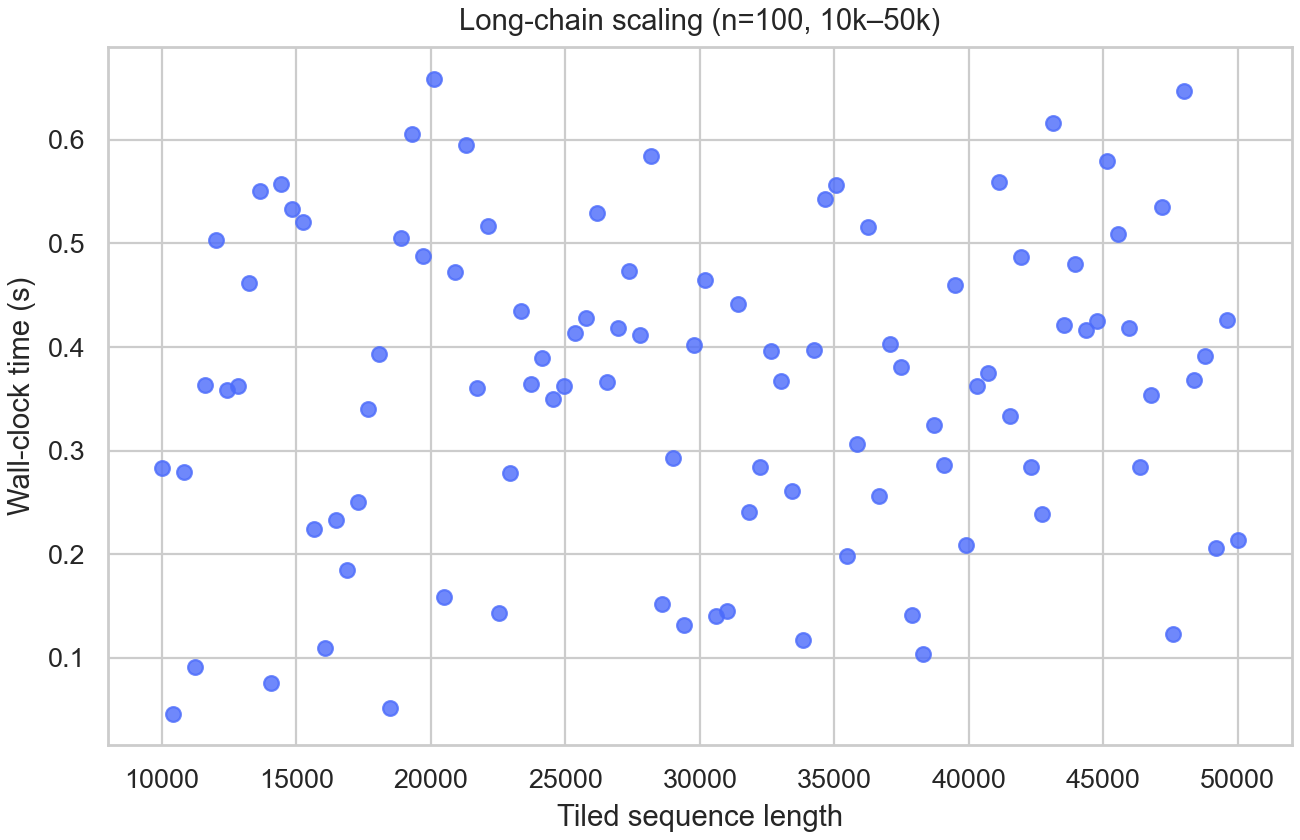
\includegraphics[width=0.72\textwidth]{benchmark_long100_time.png}
  \caption{Long100: wall-clock time versus tiled sequence length ($10\,000$--$50\,000$).}
  \label{fig:long}
\end{figure}

% ===========================================================================
\section{Discussion}
% ===========================================================================

\subsection{What PairFold does well}

PairFold demonstrates that a small, PDB-trained fragment Transformer plus careful assembly can deliver:
(i)~interpretable $(\phi,\psi)$ predictions with calibrated confidence;
(ii)~secondary-structure-aware backbones;
(iii)~near-linear scaling for long sequences; and
(iv)~explicit handling of cumulative angular error via look-ahead and local torsion descent.
These properties suit teaching tools, rapid local design loops, and streaming visualisation---settings where AlphaFold's memory footprint is the bottleneck.

\subsection{Fundamental limitations}

The central limitation remains architectural relative to MSA-conditioned folding networks:
\texttt{ContactPairNet} is sequence-only and crop-trained, so contact precision is moderate (validation precision $\approx 0.18$ at the best checkpoint with high recall), and incorrect high-scoring pairs can pull the chain away from the native basin.
Without coevolutionary pair features or recycling, PairFold still cannot consistently reach sub-$5$\,\AA\ global accuracy on compact domains.
Domain-panel RMSDs of order $\PFDomainMeanRMSD{}$\,\AA\ (class-dependent) should not be compared na\"ively to AlphaFold~2's typical low-\AA\ accuracy on the same targets~\citep{jumper2021alphafold}.

Additional limitations include:
\begin{itemize}[leftmargin=1.5em]
  \item Dependence on Chou--Fasman-style SS detection, which can misassign blocks on atypical sequences;
  \item Stochastic torsion relaxation that is not a true energy minimisation in a molecular force field;
  \item Contact anchors that are sparse and imperfect; hinge-based $\phi/\psi$ moves close distances only locally;
  \item Torsion training restricted to length $\le 5$, so medium-range motifs (e.g.\ $\beta$-turns spanning six residues) must emerge from assembly rather than from the torsion network.
\end{itemize}

\subsection{Future work}

Promising extensions that preserve PairFold's low-resource character include:
\begin{enumerate}[leftmargin=1.5em]
  \item Distilling PLM embeddings (e.g.\ small ESM-2) into the contact tower for higher precision without full MSA pipelines;
  \item Learning longer fragments ($6$--$9$-mers) or SE(3)-equivariant local frames while retaining DP segmentation;
  \item Using contact maps to rank assembly hypotheses earlier in look-ahead search, not only in post-hoc hinge relax;
  \item Finer sweeps of contact threshold, $k$, and temperature $T$ with confidence--RMSD calibration on the Domains100 panel.
\end{enumerate}

% ===========================================================================
\section{Conclusion}
% ===========================================================================

We have presented PairFold, a complete local backbone generation system that couples a fragment Transformer on $(\phi,\psi)$ with $O(N)$ segmentation, temperature-calibrated confidence, secondary-structure freezing, and look-ahead backtracking with lever-effect torsion relaxation.
On $\PFDomainN{}$ diverse domains the interactive consensus+SS path achieves mean inference time $\PFDomainMeanTime{}$\,s and mean C$\alpha$ RMSD $\PFDomainMeanRMSD{}$\,\AA; ablation on 20 domains shows the full local stack at $\approx 13.2$\,\AA; and $\PFLongN{}$ tiled chains of length $\PFLongMinLen{}$--$\PFLongMaxLen{}$ complete in $\PFLongMeanTime{}$\,s mean wall-clock.
This illustrates a clear regime: \textbf{fast, resource-light, locally plausible backbones} rather than atomic-accuracy tertiary folds.
In an era dominated by large folding networks, such local alternatives remain scientifically and practically valuable---especially when sequences grow long, hardware is modest, and the question of interest is local geometry augmented by a cheap contact prior.

% ===========================================================================
\section*{Data and software availability}
% ===========================================================================

All software components described herein (\texttt{pairfold/predict.py}, \texttt{pairfold/clash\_assembly.py}, \texttt{pairfold/structure\_blocks.py}, and the \texttt{benchmarks/} suite) are part of the PairFold workspace.
Expanded results are archived as \texttt{benchmark\_domains100.csv}, \texttt{benchmark\_long100.csv}, and \texttt{benchmark\_ablation.csv}; tables and figures are regenerated by \texttt{python benchmarks/write\_paper\_tables.py} and \texttt{python benchmarks/plot\_expanded.py}.
Experimental structures were obtained from the RCSB PDB~\citep{berman2000protein}.

% ===========================================================================
\section*{Acknowledgements}
% ===========================================================================

The authors thank the open structural biology community for publicly deposited high-resolution crystal structures that make fragment-level supervision possible, and the developers of PyTorch, BioPython, and the scientific Python stack.

% ===========================================================================
\begin{thebibliography}{99}

\bibitem{jumper2021alphafold}
Jumper, J., Evans, R., Pritzel, A., et~al. (2021).
Highly accurate protein structure prediction with AlphaFold.
\textit{Nature}, 596, 583--589.
\url{https://doi.org/10.1038/s41586-021-03819-2}

\bibitem{senior2020alphafold}
Senior, A.~W., Evans, R., Jumper, J., et~al. (2020).
Improved protein structure prediction using potentials from deep learning.
\textit{Nature}, 577, 706--710.
\url{https://doi.org/10.1038/s41586-019-1923-7}

\bibitem{lin2023evolutionary}
Lin, Z., Akin, H., Rao, R., et~al. (2023).
Evolutionary-scale prediction of atomic-level protein structure with a language model.
\textit{Science}, 379, 1123--1130.
\url{https://doi.org/10.1126/science.ade2574}

\bibitem{simons1997assembly}
Simons, K.~T., Kooperberg, C., Huang, E., \& Baker, D. (1997).
Assembly of protein tertiary structures from fragments with similar local sequences using simulated annealing and Bayesian scoring functions.
\textit{Journal of Molecular Biology}, 268, 209--225.
\url{https://doi.org/10.1006/jmbi.1997.0959}

\bibitem{rohl2004rosetta}
Rohl, C.~A., Strauss, C.~E.~M., Misura, K.~M.~S., \& Baker, D. (2004).
Protein structure prediction using Rosetta.
\textit{Methods in Enzymology}, 383, 66--93.
\url{https://doi.org/10.1016/S0076-6879(04)83004-0}

\bibitem{ramachandran1963stereochemistry}
Ramachandran, G.~N., Ramakrishnan, C., \& Sasisekharan, V. (1963).
Stereochemistry of polypeptide chain configurations.
\textit{Journal of Molecular Biology}, 7, 95--99.
\url{https://doi.org/10.1016/S0022-2836(63)80023-6}

\bibitem{engh1991accurate}
Engh, R.~A., \& Huber, R. (1991).
Accurate bond and angle parameters for X-ray protein structure refinement.
\textit{Acta Crystallographica Section A}, 47, 392--400.
\url{https://doi.org/10.1107/S0108767391001071}

\bibitem{berens2009circ}
Berens, P. (2009).
CircStat: A MATLAB toolbox for circular statistics.
\textit{Journal of Statistical Software}, 31, 1--21.
\url{https://doi.org/10.18637/jss.v031.i10}

\bibitem{chou1974prediction}
Chou, P.~Y., \& Fasman, G.~D. (1974).
Prediction of protein conformation.
\textit{Biochemistry}, 13, 222--245.
\url{https://doi.org/10.1021/bi00699a002}

\bibitem{berman2000protein}
Berman, H.~M., Westbrook, J., Feng, Z., et~al. (2000).
The Protein Data Bank.
\textit{Nucleic Acids Research}, 28, 235--242.
\url{https://doi.org/10.1093/nar/28.1.235}

\end{thebibliography}

\end{document}
